\section{Smart Pointer}
Ogni valore manipolato da un programma è memorizzato nello spazio di
indirizzamento del processo.
L'operatore \mintinline{rust}|&| e \mintinline{rust}|&mut| in Rust
permette, in C, C++ e Rust, di ottenere l'indirizzo del primo byte in
cui è memorizzato, producendo un riferimento ad un valore.
In Rust, tali riferimenti non sono puntatori nativi esposti direttamente al
programmatore, ma valori soggetti alle regole del borrow checker.

L'operazione duale, detta dereferenza (\textit{dereferencing}) o risoluzione del
riferimento, trasforma un indirizzo nel corrispondente valore referenziato. Si
utilizza l'operatore \mintinline{rust}|*| per dereferenziare esplicitamente.
Nella sintassi dei metodi, il compilatore può applicare direttamente
dereferenziazione e prestito quando appropriato.

Sia Rust che C++ permettono di ridefinire il comportamento degli operatori del
linguaggio per tipi arbitrari e di definire tipi generici, che possono essere
espansi in una molteciplità di tipo concreti, in funzione di come vengono utilizzati.


Questi meccanismi permettono di definire tipi che si usano sintatticamente in
modo simile ai puntatori, ma che aggiungono proprietà come:

\begin{itemize}
  \item \textbf{Possesso}:Garanzia di inizializzazione e rilascio.
  \item \textbf{Conteggio}: Conteggio dei riferimenti.
  \item \textbf{Mutabilità}: Mutabilità interna.
  \item \textbf{Sincronizzazione}: Sincronizzazione concorrente.
\end{itemize}

\subsection{Uso dei puntatori}
Tramite l'uso di puntatori è possibile costruire strutture dati dinamiche della
topologia non prevedibile a priori e/o variabili nel tempo come grafi, alberi,
liste. La grande libertà però espone il programmatore a problemi legati alla deduzione di
correttezza del codice che lo manipola.

Le regole restrittive imposte dal borrow checker di Rust impediscono combinazioni
di aliasing e mutabilità che renderebbero difficile garantire la sicurezza del
programma. Con soli riferimenti diventa molto difficile rappresentare strutture
cicliche persistenti.
Questa minore capacità espressiva abilita, però, analisi più approfondite ed è
alla base delle garanzie di sanità offerte dal linguaggio.


Smart pointer come \verb|Rc<T>| e \verb|Arc<T>| introducono il concetto di
possesso condiviso. Altri Smart pointer come \verb|std::rc::Weak<T>| e \verb|std::sync::Weak<T>|
introducono riferimenti privi di possesso, utili per rappresentare riferimenti
privi di possesso ed evitare cicli di possesso forte.

\section{Smart pointer in Rust}
Rust offre una varietà maggiore di smart pointer rispetto al C++, allo scopo di
coprire ulteriori casi e definire ottimizzazioni possibili nel caso specifico di
programmi puramente sequenziali piuttosto che di programmi concorrenti. Alcuni
ricalcano le astrazioni del C++ come \verb|Box|, \verb|Rc|, \verb|Arc|,
\verb|Weak|, mentre altri sono peculiari di Rust come \verb|Cell|,
\verb|RefCell|, \verb|Cow|, \verb|Mutex|, \verb|RwLock|.

Molti Smart pointer sono realizzati come strutture dati che incapsulano dati e
metadati aggiuntivi. Spesso implementano i tratti \verb|Deref| e, talvolta,
\verb|DerefMut|, per consentire un accesso al contenuto, simile a quello che
offrirebbe un puntatore. Quando un tipo implementa questi tratti, il
compilatore può usarli per rendere naturale l'accesso al contenuto.

\begin{itemize}
  \setlength{\itemsep}{1pt}
  \item \textbf{Possesso esclusivo}: \verb|Box<T>|,
  \item \textbf{Possesso condiviso}: \verb|Rc<T>|, \verb|Arc<T>|, \verb|Weak<T>|
  \item \textbf{Mutabilità condivisa}: \verb|Cell<T>|, \verb|RefCell<T>|
  \item \textbf{Sincronizzazione concorrente}: \verb|Mutex<T>|, \verb|RwLock<T>|
  \item \textbf{Clone on write}: \verb|Cow<'a, B>|
\end{itemize}

\begin{minted}[breaklines]{rust}
trait Deref {
    type Target: ?Sized;
    fn deref(&self) -> &Self::Target;
}

trait DerefMut: Deref {
    fn deref_mut(&mut self) -> &mut Self::Target;
}
\end{minted}

\subsection{\texttt{std::Box<T>}}
Struttura che possiede un valore allocato dinamicamente sullo \textit{heap}
all'atto della sua costruzione tramite \mintinline{rust}|Box::new()|.

Il dato puntato è \textbf{posseduto} dal \verb|Box|: quando esce dal proprio
scope sintattico, il blocco sullo heap viene rilasciato automaticamente tramite
il tratto \verb|Drop| (anticipabile con \mintinline{rust}|drop(b)|).

Se la struttura viene mossa in un'altra variabile, o ritornata da una funzione,
il possesso del valore allocato sullo heap passa alla destinazione che diventa
responsabile del suo rilascio.Questo rende possibile ottenere cicli di vita che si estendono oltre la durata della funzione in cui il
dato è stato creato.

Il tipo \verb|T| può avere una dimensione non nota in fase di compilazione,
ovvero non implementa il tratto\verb|Sized|. In questo caso, l'oggetto
\verb|Box<T>| diventa un \textit{fat pointer} formato da un \textbf{puntatore}
seguito da un intero di dimensione \textbf{usize} contente la lunghezza del dato
puntato.


Analogamente, se al posto del tipo concreto \verb|T| si indica con un
oggetto-tratto (\verb|dyn Trait|), si ha un fat pointer composto da due
puntatori: quello al dato sullo heap e quello a vtable del tratto.

\begin{center}
  \begin{minipage}{0.45\linewidth}
    \begin{minted}[breaklines]{rust}
let b1: Box<[i32]> = Box::new([1, 2, 3]);

let b2: Box<dyn Debug> = Box::new([1, 2, 3]);
\end{minted}
  \end{minipage}%
  \hfill
  \begin{minipage}{0.45\linewidth}
    \centering
    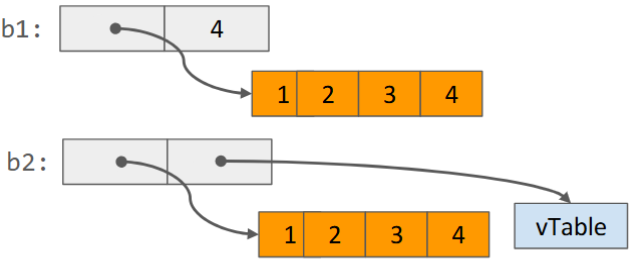
\includegraphics[width=\linewidth]{content/API_Programming/images/2026-04-21-13-26-12.png}
  \end{minipage}
\end{center}


\begin{center}
  \begin{minipage}{0.5\linewidth}
    \begin{tcolorbox}[title=Esempio di Box]
      \begin{minted}[breaklines]{rust}
fn produce(odd: bool) -> Box<i32> {
    let mut b = Box::new(0);
    if odd { *b = 5; }
    return b;
}

fn main() {
    let b1 = produce(false);
    println!("b1: {}", b1);
    let b2 = produce(true);
    drop(b1);
    println!("b2: {}", b2);
}
\end{minted}
    \end{tcolorbox}
  \end{minipage}%
  \hfill
  \begin{minipage}{0.45\linewidth}
    \centering
    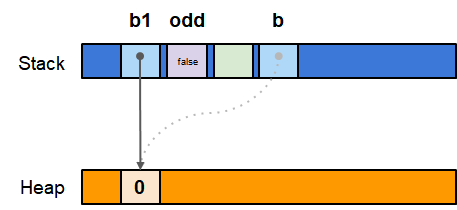
\includegraphics[width=0.75\linewidth]{content/API_Programming/images/2026-04-03-17-08-46.png}
    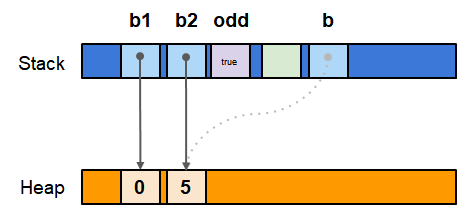
\includegraphics[width=0.75\linewidth]{content/API_Programming/images/2026-04-03-17-09-30.png}
    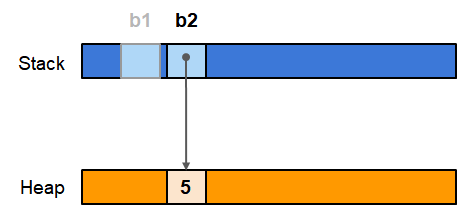
\includegraphics[width=0.75\linewidth]{content/API_Programming/images/2026-04-03-17-10-22.png}
  \end{minipage}
\end{center}


\begin{tcolorbox}
  \textbf{Nota:} b1 diventa inaccessibile già dopo la chiamata alla macro \verb|Drop|
\end{tcolorbox}



\section{Conteggio dei Riferimenti}

\subsection{\texttt{std::rc::Rc<T>}}

\begin{center}
  \begin{minipage}{0.65\linewidth}
    Quando occorre disporre di più possessori di uno stesso dato immutabile,
    si usa \verb|Rc<T>| - Resource Counted. Internamente mantiene il \textbf{dato} allocato
    e due contatori: \textbf{riferimenti forti} e \textbf{deboli}. Ad ogni
    \textbf{clonazione} del puntatore, il contatore viene \textbf{incrementato};
    \textbf{uscendo dallo scope} viene \textbf{decrementato} e, arrivato a 0, il
    blocco viene rilasciato. Non è \textit{thread-safe} per la concorrenza si
    usa \verb|Arc<T>|.


    \begin{tcolorbox}
      \textbf{Nota:} \verb|Rc<T>| si presta a realizzare alberi e grafi aciclici.
      Non può essere usato da \textbf{più di un thread}, bensì solo da programmi
      non concorrenti dato che manca di sincronizzazione interna.
    \end{tcolorbox}


  \end{minipage}%
  \hfill
  \begin{minipage}{0.3\linewidth}
    \centering
    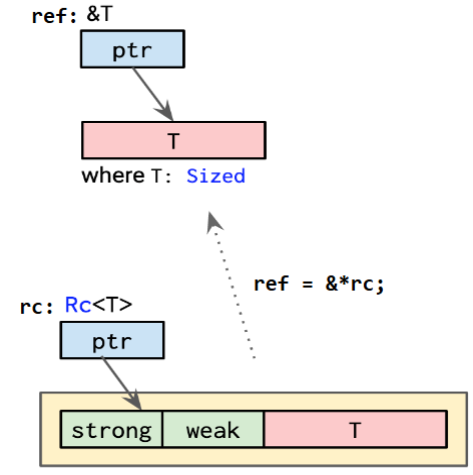
\includegraphics[width=\linewidth]{content/API_Programming/images/2026-04-03-16-46-12.png}
  \end{minipage}
\end{center}






\begin{center}
  \begin{minipage}{0.6\linewidth}
    \begin{minted}[breaklines]{rust}
enum List {
    Cons(i32, Rc<List>),
    Nil,
}

use crate::List::{Cons, Nil};
use std::rc::Rc;

fn main() {
    let a = Rc::new(Cons(5, Rc::new(Cons(10, Rc::new(Nil)))));
    let b = Rc::new(Cons(3, Rc::clone(&a)));
    let c = Rc::new(Cons(4, Rc::clone(&a)));
}
\end{minted}
  \end{minipage}%
  \hfill
  \begin{minipage}{0.35\linewidth}
    \centering
    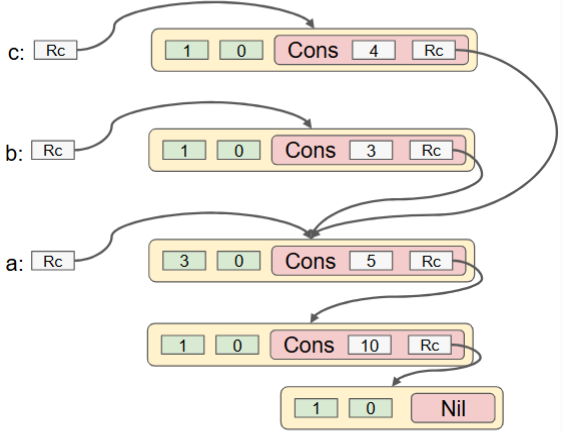
\includegraphics[width=\linewidth]{content/API_Programming/images/2026-04-03-16-48-42.png}
    \captionof{figure}{Esempio di DAG - Directed Acyclic Graph}
  \end{minipage}
\end{center}

\begin{tcolorbox}
  \textbf{Nota:} Il grafo costruito con \verb|Rc| deve essere aciclico.
\end{tcolorbox}


Per evitare problemi di omonimia con i metodi contenuti nel dato incapsulato,
tutti i metodi di Rc sono dichiarati con la sintassi estesa:

\begin{itemize}
  \item \verb|pub fn strong_count(this: &Rc<T>) -> usize|
  \item Chiamando \verb|this|, e non \verb|self|, il parametro che indica l'istanza,
        non è possibile utilizzare la notazione  puntata per invocare i metodi,
        ma occorre richiamarli nella forma estesa
  \item \verb|Rc::<T>::strong_count(&a)|
\end{itemize}

Per motivi di efficienza, l'operazione di incremento e decremento sui campi
privati \verb|strong_count| e \verb|weak_count| non è thread-safe. Per questo motivo, non è
possibile utilizzare questo smart pointer in un contesto concorrente. Esiste un
altro tipo, trattato in seguito, che supera questo limite: \verb|std::sync::Arc<T>|

\subsubsection{Mutare il contenuto di Rc<T>}

Un valore di tipo \textbf{Rc<T>} non offre normalmente accesso mutabile diretto
al contenuto.

\begin{itemize}
  \item Il metodo \mintinline{rust}|Rc::get_mut(&mut rc)-> Option<&mut T>|
        restituisce un riferimento mutabile se e solo se rc è l'unico riferimento
        forte al valore, altrimenti restituisce \verb|None|
  \item Il metodo
        \mintinline{rust}|Rc::make_mut(&mut rc) -> &mut T| restituisce sempre un
        riferimento mutabile: tuttavia, se esistono altri riferimenti forti, il valore
        verrà prima clonato, così da lasciare invariato quanto conosciuto dagli altri
        possessori
\end{itemize}

Quando occorre mutabilità condivisa senza effettuare delle copie, si usa
tipicamente \verb|Rc<RefCell<T>>|.


\begin{minted}[breaklines]{rust}
use std::rc::Rc;

let mut a = Rc::new(String::from("abc"));

if let Some(s) = Rc::get_mut(&mut a) {s.push('!');}

assert_eq!(&*a, "abc!");  // a = rc *rc = stringa &*a = slice

let mut x = Rc::new(String::from("hello"));
let y = x.clone();

Rc::make_mut(&mut x).push('!');

assert_eq!(&*x, "hello!");
assert_eq!(&*y, "hello");
\end{minted}


\subsection{\texttt{std::rc::Weak<T>}}
Se si costruisse una sequenza circolare di puntatori con \verb|Rc<T>|, la memoria non
potrebbe più essere rilasciata.
Come nel caso di \verb|shared_ptr| in C++, la catena dei puntatori terrebbe in vita
tutti i blocchi, garantendo che il conteggio dei riferimenti valga almeno 1.


È possibile rappresentare back-reference e dipendenze cicliche senza introdurre
cicli di possesso forte utilizzando il tipo \verb|Weak<T>|.
Esso è una versione di \verb|Rc<T>| che contiene un riferimento senza possesso
al blocco allocato.

Si crea un valore di tipo \verb|Weak<T>| a partire da un \verb|Rc<T>| con il
metodo \mintinline{rust}|Rc::downgrade(&rc)|.

Se il valore originale è ancora in vita, ovvero se \textbf{strong\_count() > 0},
è possibile costruite un nuovo valore di tipo \verb|Rc<T>| invocando il
metodo \mintinline{rust}|upgrade()|, che restituisce un \textbf{Option<Rc<T>>}.


\begin{minted}[breaklines]{rust}
use std::rc::Rc;

let five = Rc::new(5);
let weak_five = Rc::downgrade(&five);
let strong_five: Option<Rc<_>> = weak_five.upgrade();
assert!(strong_five.is_some());

// Destroy all strong pointers.
drop(strong_five);
drop(five);

assert!(weak_five.upgrade().is_none());
\end{minted}

\begin{tcolorbox}
  \textbf{Note:} Il tipo \verb|Weak<T>| offre il supporto per la costruzione di strutture dati cicliche non possibile con \verb|Rc<T>|
\end{tcolorbox}



\section{Interior Mutability}


\subsection{\texttt{std::cell::Cell<T>}}

\begin{center}
  \begin{minipage}{0.75\linewidth}
    In condizioni normali, Rust consente o più riferimenti condivisi
    immutabili, oppure un unico riferimento mutabile. Esistono situazioni in cui
    l'analisi statica eseguita in fase di compilazione è troppo restrittiva.


    Tuttavia, il modulo \verb|std::cell| offre contenitori per
    \textit{mutabilità condivisa e controllata} in contesti single-thread. È
    possibile cioè avere più riferimenti al valore pure essendo in grado di
    mutarlo. I tipi offerti possono funzionare solo in contesti non concorrenti
    (basati su singolo thread).


    La struct \verb|std::cell::Cell<T>|implementa la mutabilità
    del dato contenuto al suo interno attraverso metodi che non richiedono la
    mutabilità del contenitore. Consente accessi per copia/sostituzione del
    contenuto. Si dice che Cell implementa un meccanismo di \textbf{interior mutability}
  \end{minipage}%
  \hfill
  \begin{minipage}{0.2\linewidth}
    \centering
    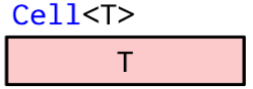
\includegraphics[width=\linewidth]{content/API_Programming/images/2026-04-03-16-52-31.png}
  \end{minipage}
\end{center}



\begin{minted}[breaklines]{rust}
use std::cell::Cell;
struct SomeStruct {
    a: u8,
    b: Cell<u8>,
}

let my_struct = SomeStruct { a: 0, b: Cell::new(1) };
// my_struct.a = 100; // ERRORE: `my_struct` è immutabile
my_struct.b.set(100); // OK: anche se `my_struct` è immutabile, `b` è una Cell e può essere modificata/assert_eq!(my_struct.b.get(), 100);
assert_eq!(my_struct.b.get(), 100);
\end{minted}

\subsubsection{Metodi di Cell<T>}

\begin{itemize}
  \item \verb|get(&self) -> T| - restituisce il dato contenuto al suo interno, a condizione che T implementi il tratto Copy
  \item \verb|take(&self) -> T| - restituisce il valore contenuto,
        sostituendolo con il risultato dell'invocazione di \verb|Default::default()|. A
        condizione che T implementi il tratto \textbf{Default} che permette la costruzione di un valore predefinito
  \item \verb|replace(&self, val: T) -> T| - sostituisce il valore contenuto
        nella cella con quello passato come parametro e lo restituisce come risultato. Questo metodo non pone restrizioni sul tipo di dato
  \item \verb|into_inner(self) -> T| - consuma la cella e restituisce il
        valore contenuto. Anche in questo caso, può essere usato con ogni tipo di
        dato
\end{itemize}

\begin{tcolorbox}
  \textbf{Nota:} Come \verb|Rc<T>|, non è possibile utilizzarlo in un contesto concorrente.
\end{tcolorbox}


\subsection{\texttt{std::cell::RefCell<T>}}

\begin{center}
  \begin{minipage}{0.75\linewidth}
    Simula riferimenti condivisi e mutabili verificati in fase di esecuzione (a runtime) anziché compilazione.
    Tentativi di violazione (es. chiamare \mintinline{rust}|borrow_mut()| mentre c'è già un prestito) generano \verb|panic|.

  \end{minipage}%
  \hfill
  \begin{minipage}{0.2\linewidth}
    \centering
    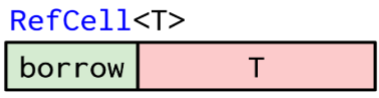
\includegraphics[width=\linewidth]{content/API_Programming/images/2026-04-03-16-53-49.png}
  \end{minipage}
\end{center}

\verb|Cell<T>| non consente di creare riferimenti al dato contenuto al suo interno, ma
solo di inserire, estrarre o sostituire il valore.


La struct \verb|std::cell::RefCell<T>| consente di ottenere oggetti (guardie)
che si comportano come riferimenti (condivisi o mutabili) al contenuto, con
regole di prestito verificate all'atto dell'esecuzione e non in compilazione.
Eventuali tentativi di violazione delle regole generano una condizione di panic.

\subsubsection{Metodi di RefCell<T>}

\begin{itemize}
  \item \verb|borrow(&self) -> Ref<'_, T>| - restituisce una guardia che si
        comporta come un riferimento condiviso. Oppure provoca un panic se è già
        presente un riferimento mutabile.
  \item \verb|borrow_mut(&self) -> RefMut<'_, T>| - restituisce una guardia
        che si comporta come un riferimento mutabile. Oppure provoca un panic se è
        già presente un riferimento semplice.
\end{itemize}

\begin{tcolorbox}
  \textbf{Note:} Il programma può andare in panic se si tenta di violare le regole di prestito.
\end{tcolorbox}


\begin{minted}[breaklines]{rust}
use std::cell::RefCell;
let c = RefCell::new(5);
{
    let mut m = c.borrow_mut();
    assert!(c.try_borrow().is_err());
    *m = 6;
}

{
  let m = c.borrow();
  assert!(c.try_borrow().is_ok());
  assert!(*m == 6);
}

assert_eq!(*c.borrow(), 6);
\end{minted}

% \section{Altri Smart Pointer e Metodi}
\subsection{\texttt{std::borrow::Cow<'a, B>}}
Smart pointer che implementa il meccanismo \textit{clone on write} tramite \verb|enum| (\verb|Borrowed|, \verb|Owned|) .
Se si modifica un dato condiviso, il dato viene clonato: si prende possesso
della copia e si effettua la modifica, lasciando l'originale invariato;
Altrimenti se il dato che si vuole modificare era già posseduto,
si modifica direttamente l'originale.


Implementato sotto forma di enumerazione:

\begin{minted}[breaklines]{rust}
pub enum Cow<'a, B>
where B: 'a + ToOwned + ?Sized,
  {
    Borrowed(&'a B),
    Owned(<B as ToOwned>::Owned),
  }
\end{minted}

Si istanzia attraverso il metodo \mintinline{rust}|Cow::from(...)|

In base al dato da incapsulare, viene scelta la variante \textbf{Owned} o \textbf{Borrowed}.


\begin{center}
  \begin{minipage}{0.45\linewidth}
    \begin{minted}[breaklines]{rust}
use std::borrow::Cow;
// Riusa la slice se non occorre
// effettuare modifiche
// Altrimenti, alloca una nuova String
fn normalize_whitespace(line: &str) -> Cow<'_, str> {
  if line.contains('\t') {
    Cow::Owned(line.replace('\t', " "))
  } else {
   Cow::Borrowed(line)
  }
}
\end{minted}
  \end{minipage}%
  \hfill
  \begin{minipage}{0.45\linewidth}
    \begin{minted}[breaklines]{rust}
fn main() {
  let a = "INFO user=alice op=login";
  let b = "WARN\tuser=bob\top=logout";
  let na = normalize_whitespace(a);
  let nb = normalize_whitespace(b);
  println!("a -> {}", na);
  println!("b -> {}", nb);

  assert!(
  matches!(na,Cow::Borrowed(_)));

  assert!(
  matches!(nb, Cow::Owned(_)));
}
\end{minted}
  \end{minipage}
\end{center}

\subsection{Smart pointer e metodi (\texttt{self})}

Nella firma di un metodo, è possibile utilizzare, oltre a \textit{self} ed alle sue
variazioni, anche \verb|Box<Self>|, \verb|Rc<Self>|, o \verb|Arc<Self>|.
In tal caso, il metodo può essere solo invocato a partire dal corrispondente
tipo di puntatore.
L'invocazione del metodo passa la proprietà del puntatore al metodo stesso.

A differenza di quanto accade con i riferimenti, non è disponibile una forma
abbreviata per la sintassi di \textit{self}.
In questi casi il tipo del receiver deve essere dichiarato esplicitamente, ad
esempio, \verb|self: Rc<Self>|.

\begin{minted}[breaklines]{rust}
impl Node {
    fn append_to(self: Rc<Self>, parent: &mut Node) {
        parent.children.push(self);
    }
}
\end{minted}



\section{Esempio: Albero doppiamente collegato}
Un albero dove i nodi figli conoscono il padre e viceversa si implementa combinando \verb|Rc|, \verb|RefCell| e \verb|Weak|.

\begin{figure}[h!]
  \centering
  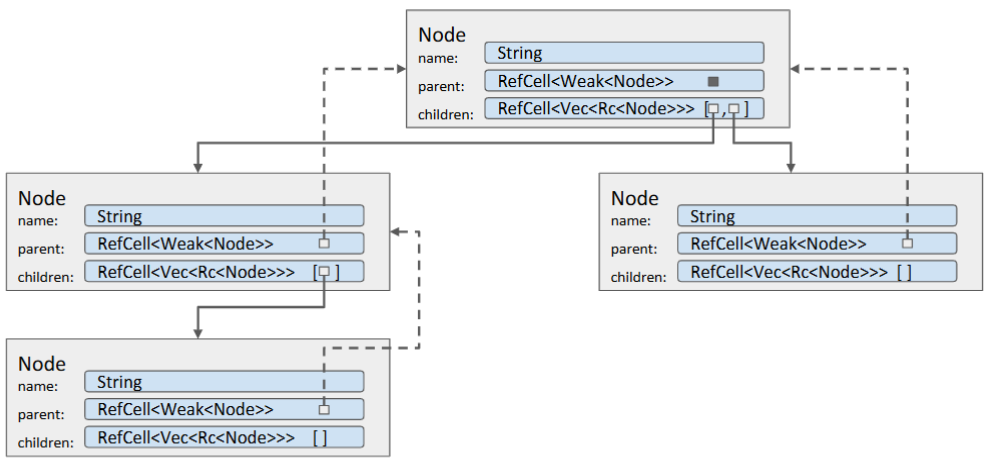
\includegraphics[width=0.45\linewidth]{content/API_Programming/images/2026-04-03-16-33-26.png}
\end{figure}

\begin{minted}[breaklines]{rust}
use std::cell::RefCell;
use std::rc::{Rc, Weak};

#[derive(Debug)]
struct Node {
    name: String,
    parent: RefCell<Weak<Node>>,
    children: RefCell<Vec<Rc<Node>>>,
}

impl Node {
    fn new(name: &str) -> Rc<Self> {
        Rc::new(Node {
            name: name.to_string(),
            parent: RefCell::new(Weak::new()),
            children: RefCell::new(Vec::new()),
        })
    }

    fn add_child(parent: Rc<Node>, child: Rc<Node>) {
        *child.parent.borrow_mut() = Rc::downgrade(&parent);
        parent.children.borrow_mut().push(child);
    }

    fn print_tree(node: &Rc<Node>, depth: usize) {
        println!("{}{}", " ".repeat(depth * 2), node.name);
        for child in node.children.borrow().iter() {
            Node::print_tree(child, depth + 1);
        }
    }
    fn get_root(node: &Rc<Node>)-> Rc<Node> {
        let mut n = node.clone();
        loop {
            let parent = n.parent.borrow().upgrade();
            match parent {
                Some(p) => n = p.clone(),
                None => break,
            }
        }
    
    }
    fn main() {
        let root = Node::new("root");
        let child1 = Node::new("child1");
        let child2 = Node::new("child2");
        Node::add_child(root.clone(), child1.clone());
        Node::add_child(root.clone(), child2);
        Node::add_child(child1.clone(), Node::new("subchild"));
        Node::print_tree(&Node::get_root(&child1), 0);
    }
}

//root
//  child1
//      subchild
//  child2
\end{minted}


\section{Cheat Sheet dei Container in Rust}
Per facilitare la comprensione del layout in memoria dei vari container e puntatori intelligenti:

\begin{figure}[h!]
  \centering
  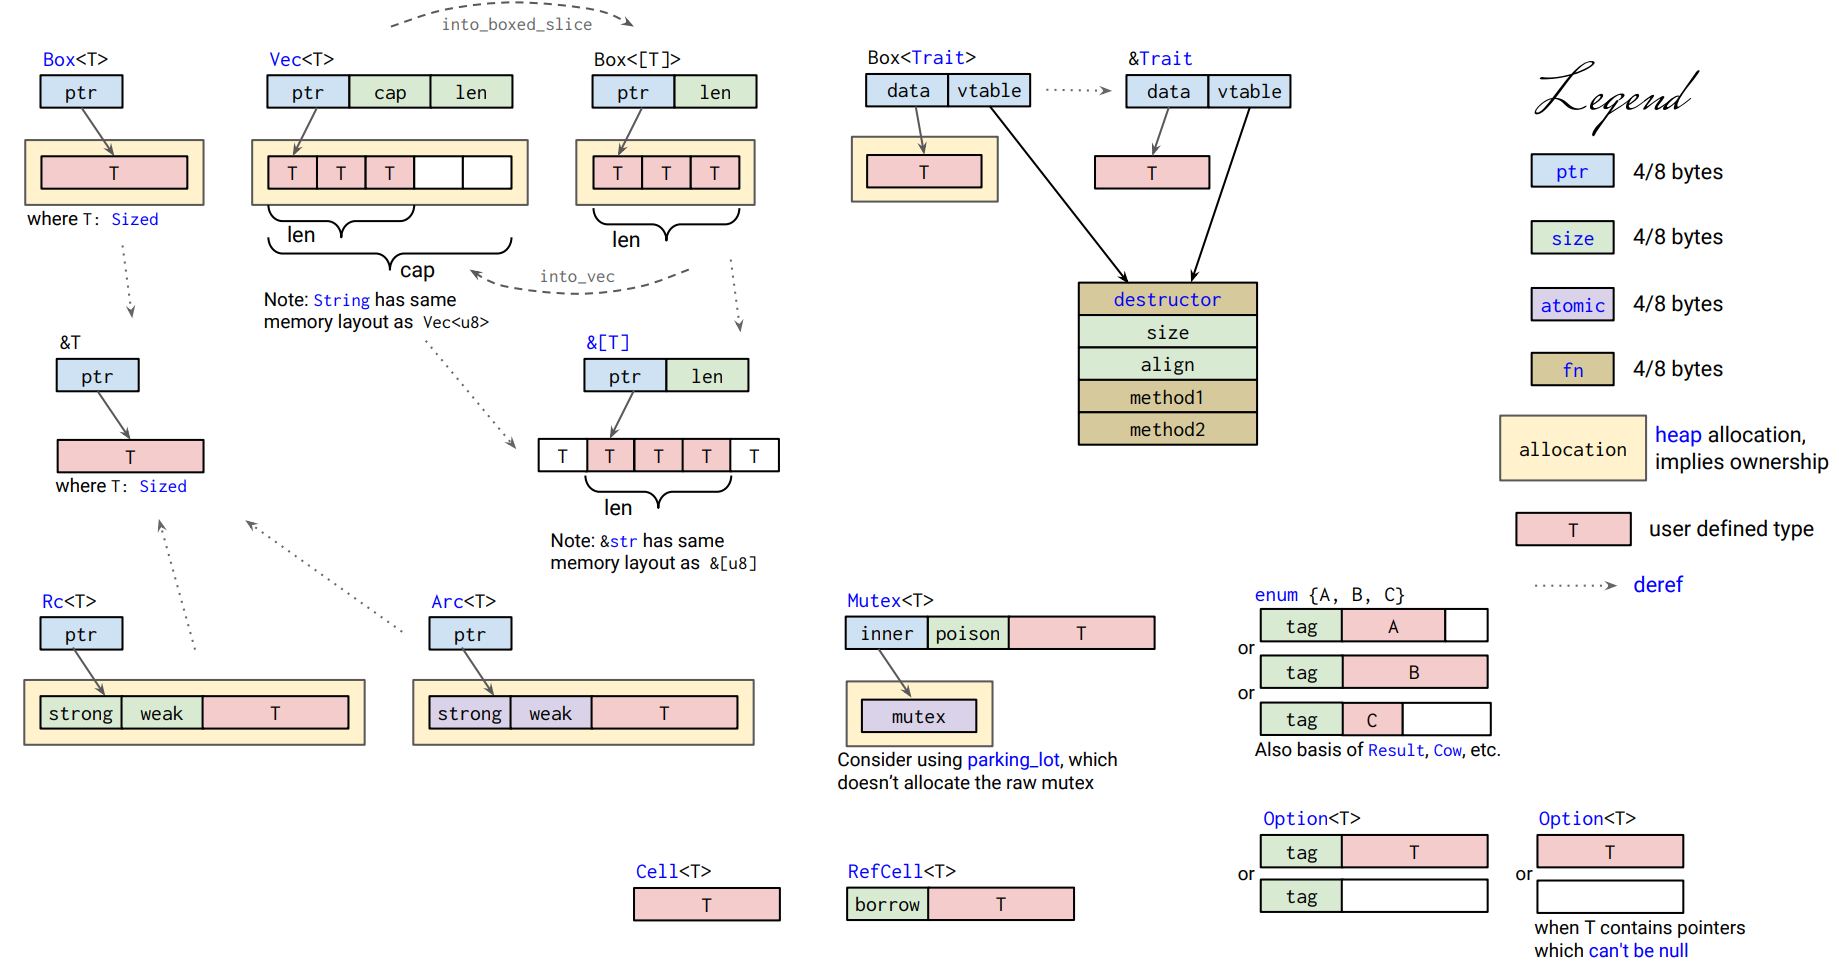
\includegraphics[width=1\linewidth]{content/API_Programming/images/2026-04-03-16-31-58.png}
\end{figure}